\chapter{ОПИСАНИЕ ВЫБОРКИ}

В качестве объектов исследования выступают файлы сложного формата \textbf{doc}.
Данный вид файлов используется для хранения текстовой и графической информации, а основным программным продуктом, позволяющим их создавать и редактировать, является Microsoft Word.
Документы данного формата внутри имеют бинарную структуру, схожую по строению со структурой файловых систем. \cite{doc_format}

Как было сказано, основной задачей данной работы является описание и построение алгоритма, способного самостоятельно и в автоматическом режиме определять степень вредоносности файлов формата \textbf{doc}.
Для достижения данной цели мы будем использовать комбинацию известных алгоритмов, позволяющих учитывать предыдущий опыт -- так называемых обучаемых алгоритмов.
В нашем случае под предыдущим опытом стоит понимать наличие информации о двух наборах файлов: множество безопасных для работы документов и множество вредоносных документов.
Объединение этих двух наборов мы в дальнейшем будем называть выборкой объектов, подразумевая, что файлы были получены из некоторого нам неизвестного распределения всех возможных файлов формата \textbf{doc}. 
Процесс получения данных наборов называется разметкой, и почти всегда данный процесс происходит в ручном режиме.
Тем не менее, обычно нас не интересует, каким способом было получено разделение файлов на разные типы, но при этом для нас очень важно, что вероятность ошибочного размещение документа в не подходящем классе была близка к нулю, иначе, основываясь на плохо размеченной выборке объектов, мы можем создать ошибочную модель, допускающую при работе заметное число ошибок.

В отличие от ручного анализа, когда все действия, выполняемые программой при работе с документом, анализируются человеком, нам для успешного создания работающей модели важно наличие файлов различных типов.
Таким образом, в качестве первого шага, мы опишем состав нашей выборки объектов, информацию о которых в дальнейшем будем использовать как исходные данные для алгоритмов обучения.

\section{Вредоносные файлы}

На данный момент известно огромное множество видов вредоносных программ.
Также существуют различные формальные классификации, позволяющие присвоить метку почти любому вредоносному объекту: от игрушечных программ-шуток до целенаправленного высокотехнологичного программного оружия.

Под вредоносной программой принято подразумевать файл исполняемого формата, например \textbf{exe}, при запуске которого управление получает код, выполняющий несанкционированные действия относительно пользователя или владельца компьютера. 
Данный способ, захватывающий поток исполнения, довольно надёжен, но при этом имеет весьма существенный и неустранимый недостаток -- пользователь должен собственноручно инициировать начало исполнения кода.
Также такой сценарий захвата через исполняемый файл хорошо изучен в мире, что уменьшает шансы успешного прохождения возможного барьера из современных антивирусов.
В нашем случае объектом исследования являются файлы формата \textbf{doc}, предназначенные для хранения и отображения текстовой информации. 
Ожидаемым поведением при открытии файла такого формата является отображение текста, но никак не запуск произвольного и неконтролируемого программного кода.
Данный факт значительно увеличивает процент людей, которые будут успешно атакованы.

Главной причиной, дающей возможность злоумышнику исполнять произвольный код при работе с неисполняемыми объектами, являются ошибки, допущенные при написании исходного кода программ, непосредственно взаимодействующих с пользовательскими файлами. 
Для объектов формата \textbf{doc} существует несколько таких программ.
Мы будем исследовать только работу Microsoft Word.
С момента первого выпуска данного текстового процессора были найдены десятки подобных ошибок, чем успешно пользуются многие авторы вирусов.
Одной из таких ошибок, например, является недостаточная или неполная проверка данных, вводимимых пользователем тем или иным способом через документ.
Забытая проверка на максимальную длину для введённой строковой последовательности выливается в размещение данных в блоке памяти, имеющем меньший размер, чем необходимо. 
Таким образом, ввиду особенностей организации хранения служебной информации в современном компьютере, злоумышленник получает возможность видоизменять её и в итоге влиять на поток исполнения исходной программы.
Данная техника называется атакой на переполнение буфера и широко применяется в сфере компьютерной безопасности.

Работу такого вида вирусов можно разделить на следующие этапы:

\begin{itemize}
\item эксплуатирование ошибки
\item работа промежуточного машинного кода
\item работа основной функциональности вируса
\end{itemize}

В виду ограничений, возникающих во время использования уязвимости, очень редко удаётся выполнить необходимые действия сразу же после перехода на программный код злоумышленника.
Поэтому после эксплуатация ошибки управление получает промежуточный машинный код, именуемый шелл-кодом.
Задачей шелл-кода является подготовка пользовательского окружения для запуска основной функциональности вируса.
В основном промежуточный код либо производит распаковку дополнительных данных из \textbf{doc} файла, либо скачивает основную часть функциональности вируса через локальную или глобальную сеть.
Таким образом шелл-код предоставляет модульность работы вредоносного кода, то есть работа промежуточного кода и работа основного кода может быть не связана.
Более того, каждый из этих этапов зачастую реализован разными людьми.

В исследуемую выборку были отобраны файлы, работающие описанным выше образом.
Процесс формирования такого набора объектов занял продолжительное время, так как в основном осуществлялся в ручном режиме.
Также обязательным условием была полная работоспособность файла в лабораторных условиях.
Всего было отобрано 15 вреодосных программ.

Мною было произведено дизассемблирование нескольких объектов, с целью более подробного изучения работы шелл-кода после эксплуатирования уязвимостей.
Ниже будет описана работа одного из проанализированных примеров.
В качестве инструментов выступали IDA Pro Free\footnote{https://www.hex-rays.com/products/ida/} и OllyDbg\footnote{http://www.ollydbg.de}.

\newpage
\section{Обзор работы шелл-кода}

В данном примере шелл-код получает управление после использования ошибки в обработке таблицы шрифтов.
Её структура отображена на рисунке 1.1. 

\begin{figure}[ht]
	\centering
    \begin{subfigure}[b]{1\textwidth}
    \centering
        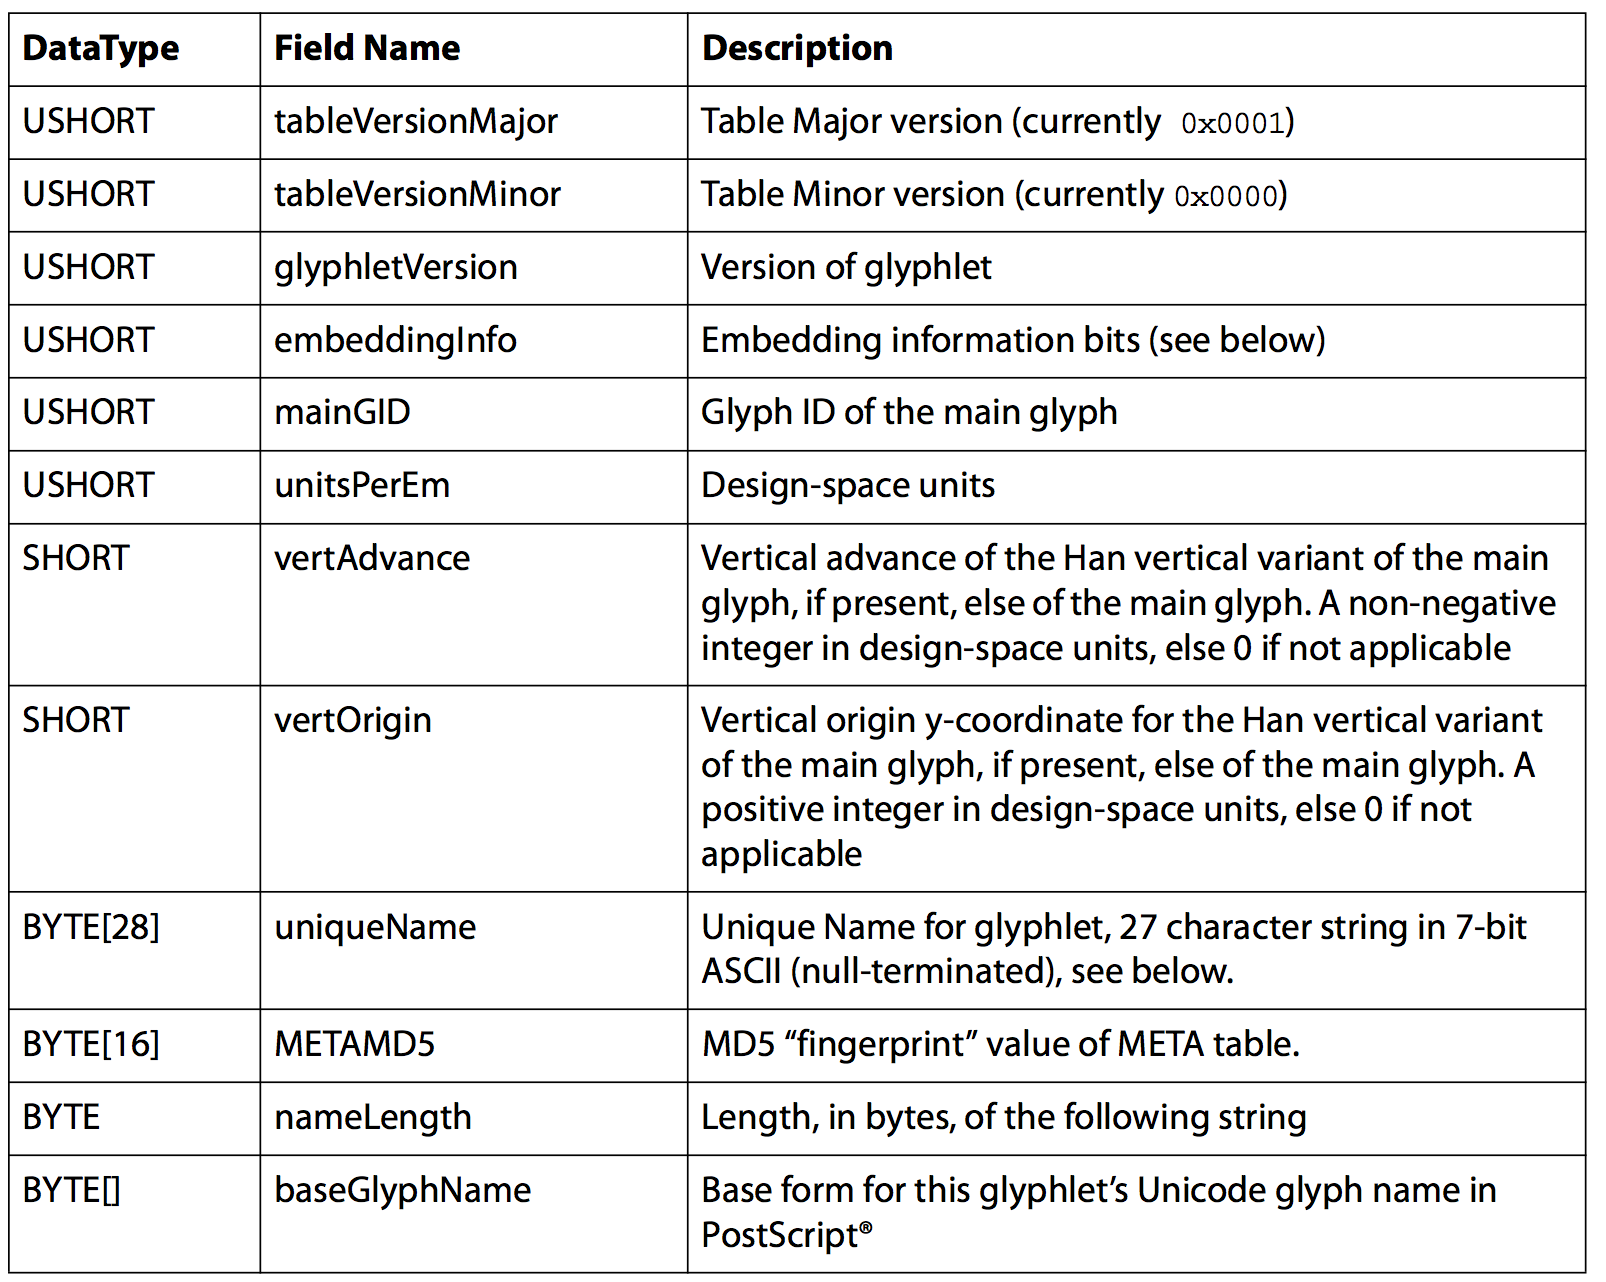
\includegraphics[scale=0.5]{1.pdf/pasted-image-15.png}
    \end{subfigure}
 
    \caption{Формат таблицы шрифтов SING}
    \label{fig_parsetree}
\end{figure}

Как можно видеть из рисунка, на поле с названием \textbf{uniqueName} отводится ровно 28 байт, включаю конечный нулевой байт.
Из-за забытой проверки на длину данного поля, мы можем передавать произвольной длины названия шрифтов и изменять адрес возврата функции.

Мною также был извлечён интерпретируемый код, который исполняется во время отрытия файла.
Он наполняет большую часть виртуальной памяти процесса вредоносным шелл-кодом, чтобы на него было легче попасть в момент передачи управления.
Данная технология известна в мире как HeapSpray. \cite{heap_spray}
С содержимым интерпретируемого кода можно ознакомиться в приложении А.

Первым делом работающий шелл-код получает адреса системных функций, необходимых ему для дальнейшей работы.
Это происходит с помощью сканирования заранее известных таблиц расположенных в памяти каждого процесса. \cite{peb_ldr}\cite{peb_ldr_example}
Адреса следующих функций были извлечены и запомнены шелл-кодом:
\begin{itemize}
\item kernel32.ExitProcess
\item kernel32.GlobalFree
\item kernel32.GetCommandLineA
\item kernel32.WinExec
\item kernel32.\_lwrite
\item kernel32.\_lcreat
\item kernel32.GetTempPathA
\item kernel32.CloseHandle
\item kernel32.GlobalAlloc
\item kernel32.ReadFile
\item kernel32.SetFilePointer
\item kernel32.GetFileSize
\end{itemize}

Далее шелл-коду необходимо идентифицировать файл в котором он располагается.
Это происходит с помощью перебора открытых файловых дескрипторов, являющимся неотрицательным целым числом.
Для каждого такого дескриптора происходит получение размера открытого файла и сравнение с эталонным.

\newpage
Данный шаг достигается с помощью выполнения ассемблерного кода, изображённого на рисунке 1.2. 

\begin{figure}[ht]
	\centering
    \begin{subfigure}[b]{1\textwidth}
    \centering
        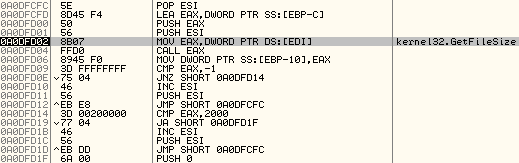
\includegraphics[scale=0.8]{1.pdf/pasted-image-19.png}
    \end{subfigure}
 
    \caption{Поиск по открытым файловым дескрипторам}
    \label{fig_parsetree}
\end{figure}

Как только первый шаг поиска был пройден, производится дополнительная проверка по сигнатуре в файле.
Всего проверяется две четырехбайтные сигнатуры, имеющие значения \textbf{0x44506450} и \textbf{0xAEEAFEEF}
Код проверки сигнатур можно увидеть на рисунке 1.3.

\begin{figure}[ht]
    \centering
    \begin{subfigure}[h]{0.6\textwidth}
    \centering
        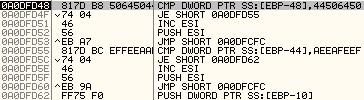
\includegraphics[scale=0.7]{1.pdf/pasted-image-25.png}
        \caption{}
        \vspace*{5mm}
    \end{subfigure}
    \begin{subfigure}[h]{0.6\textwidth}
    \centering
        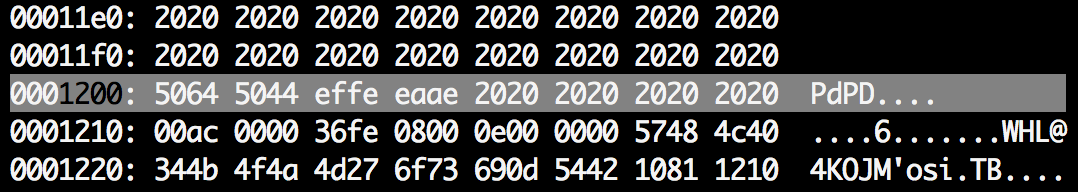
\includegraphics[scale=0.7]{1.pdf/pasted-image-27.png}
        \caption{}
    \end{subfigure}
    \caption{(а) Код проверки сигнатуры; (б) Байты сигнатур в исходном файле}
    \label{fig_parsetree}
\end{figure}

После того как шелл-код проверил правильность исходного файла, происходит распаковка второй части вируса.
Распаковка содержит следующие этапы работы шелл-кода:
\begin{itemize}
\item позиционирование указателя для считывания в файле
\item чтение зашифрованной второй части
\item расшифровывание с помощью примитивной операции исключающего \textbf{ИЛИ}
\item получение пути до системной директории, содержащей временные файлы
\item создание и запись второй части вируса
\item запуск второй части вируса
\item аварийный выход программы
\end{itemize}

Ассемблерный код, выполняющий каждый из этих этапов представлен на рисунке 1.4.
\newpage
\begin{figure}[ht]
    \centering
    \begin{subfigure}[h]{0.6\textwidth}
    \centering
        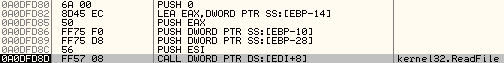
\includegraphics[scale=0.7]{1.pdf/pasted-image-31.png}
        \caption{}        
    \end{subfigure}
    \begin{subfigure}[h]{0.6\textwidth}
    \centering
        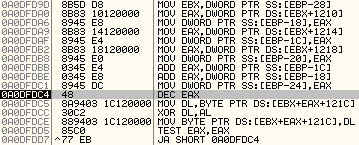
\includegraphics[scale=0.7]{1.pdf/pasted-image-33.png}
        \caption{}
      
    \end{subfigure}
    \begin{subfigure}[h]{0.6\textwidth}
    \centering
        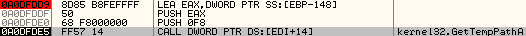
\includegraphics[scale=0.7]{1.pdf/pasted-image-35.png}
        \caption{}
        
    \end{subfigure}
    \begin{subfigure}[h]{0.6\textwidth}
    \centering
        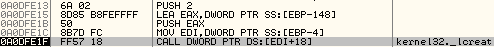
\includegraphics[scale=0.7]{1.pdf/pasted-image-37.png}
        \caption{}
        
    \end{subfigure}
    \begin{subfigure}[h]{0.6\textwidth}
    \centering
        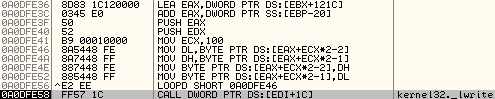
\includegraphics[scale=0.7]{1.pdf/pasted-image-39.png}
        \caption{}
        
    \end{subfigure}        
    \begin{subfigure}[h]{0.6\textwidth}
    \centering
        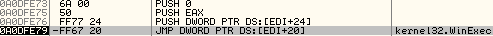
\includegraphics[scale=0.7]{1.pdf/pasted-image-41.png}
        \caption{}
        
    \end{subfigure}         
    \begin{subfigure}[h]{0.6\textwidth}
    \centering
        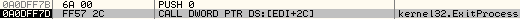
\includegraphics[scale=0.7]{1.pdf/pasted-image-43.png}
        \caption{}
    \end{subfigure}
    \caption{Этапы распаковки второй части вируса}
    \label{fig_parsetree}
\end{figure}


После анализа нескольких подобных примеров, можно выделить два основных этапа работы вредоносной программы:
\begin{itemize}
\item подготовительный этап для запуска шелл-кода
\item непосредственное исполнение шелл-кода
\end{itemize}

Во время подготовительного этапа, в нашем случае это работа кода, реализующего HeapSpray, атакуемая программа ведёт себя крайне нестабильно: зависает, начинает занимать слишком большие области памяти.
С другой стороны второй этап можно определить по аномальной последовательности системных вызовов.
Оба этих этапа послужат отправной точкой для создания статистических моделей в следующих главах.

\section{Безопасные файлы}

Чтобы построенная модель могла определять степень вредоносности объектов, ей при построении необходимо в дополнение к информации, полученной по вредоносным файлам, подать на вход данные, собранные по безвредным объектам.
В отличие от вредоносных объектов, безвредные объекты могут быть созданы непосредственно с помощью текстового редактора Microsoft Word.
Так как выборка должна иметь конечный размер, нам необходимо ограничить набор безвредных файлов, которые попадут в исходные данные для обучения.
При этом нам нужно добиться разнообразия среди файлов.

Основной идеей было выделение основных характеристик документа и объединения их значений в различных комбинациях.
Такими характеристиками были выбраны следующие позиции:
\begin{itemize}
\item количество страниц
\item вариант используемого шрифта
\item наличие таблиц
\item наличие встроенной графики
\item наличие графических изображений
\item использование нестандартных стилей
\item визуальное форматирование текста
\end{itemize}

Перечисленный набор характеристик представляется достаточным для построения выборки разнообразных безопасных файлов и был принят в качестве отправной точки.
Анализ результатов работы, а так же более подробный обзор функциональности программного обеспечения Microsoft Word и дальнейшая кластеризация характеристик безопасных файлов могут повысить качество создаваемой модели.
Для сохранения баланса между безвредными и вредоносными файлами было создано 15 безопасных объектов.